\documentclass[../rzero]{subfiles}
\begin{document}
\chapter{Energy In General Relativity}\label{energyGeneralRelativityChapter}

\begin{chapquote}{From Nathan Rosen\cite{rosenEnergyUniverse1994}}
``The energy of the universe, including the energy of the matter and that of the gravitational field, is investigated with the help of the Einstein gravitational pseudo-tensor. It is found that the total energy vanishes.''
\end{chapquote}


\section{Einstein had a problem}
The Einstein theory of General Relativity is missing something. Energy.

Einstein, in a lecture delivered on 9 September 1913 to the 96th annual meeting of the Swiss Society for Natural Sciences in Frauenfeld (translated)\cite{naturforschende1914vierteljahrsschrift}: 

Imagine this live and in person: 
\begin{quotation}
	It has already been emphasized above that the material process alone cannot satisfy the conservation laws; but we must demand that the conservation laws be satisfied for the material process and the gravitational field \textit{together}. 
\end{quotation}

A minute or so later he follows up with: 

\begin{quotation} 
...that along with the stress-energy components $T_{\sigma \nu}$ of the material process, those of the gravitational field (namely, $t_{\sigma \nu}$) appear as an equivalent field-inducing cause, a circumstance that obviously must be demanded; for the gravitational effect of a system may not depend on the \textit{physical nature} of the system's field-producing energy.\footnote{See the  \href{https://einsteinpapers.press.princeton.edu/vol4-trans/208}{Princeton papers}.}
\end{quotation}

Note the word 'obviously'. Still, Einstein had to drop this \textit{obvious} - that the energy of the gravitational field should feedback into the equations, in order to ship General Relativity in late 1915. The reason for this was that his energy tensor $t_{\sigma \nu}$ turned out not to be a tensor, but a rather a pseudo tensor. It isn't covariant.  

Fast forward to today: Field energy in General Relativity is a mess. No proper covariant energy tensor has been found, most likely because it's impossible. The fix presented here is not a normal one, we're going to abandon covariance. But first the mess.

\section{The Mess}
\subsection{Gravitational Field Energy Does Not Exist}
Misner Thorne and Wheeler\cite{Wheeler1973}:
   
   \begin{quotation}
   Anybody who looks for a magic formula for ``local gravitational energy-momentum'' is looking for the right answer to the wrong question. Unhappily, enormous time and effort were devoted in the past to trying to ``answer this question'' before investigators realized the futility of the enterprise. Toward the end, above all mathematical arguments, one came to appreciate the quiet but rock-like strength of Einstein's equivalence principle. One can always find in any given locality a frame  of reference in which all local ``gravitational fields'' ... disappear.
   \end{quotation}
   
 The cope that people use to enable this is to simply shrug and say gravitational energy is not conserved. But MTW are saying more - they are saying that it doesn't exist. Read it again - at every point in a manifold, one can come up with a frame of reference where energy does not exist. Making \textit{that} your frame this frame zeros out the energy. Of course MTW on that same page wiggle out of their statement, using what I call $The\ Hack^{TM}$
 
 \subsection{The Hack}
 The solution used for this problem is for researchers to just 'know' when to bundle up some region of gravitational field energy and toss it into $T_{\sigma \nu}$. A mess. Sure it has a set of rules and makes sense - but lets get this out in the open, it's not automatic in the equations of General Relativity, as it should obviously be.
 
  \subsection{Quasi Local Energy}
  Szabados has a great review article on Quasi-Local energy.\cite{szabadosQuasiLocalEnergyMomentumAngular2009}. I note that it's pretty obvious that there is a huge problem with energy in General Relativity when a huge review paper can't simply state where it is and how to calculate it. 
  In the last five or so decades, the use of quasi-local energy has come in as a useful tool to imagine the energy in a gravitational solution. Consider what the titans of General Relativity say about the location of the gravitational energy in the simplest solution out there, the Schwarzschild:
  (!!!get references!!!) 
  \begin{enumerate}
  	\item Penrose: The energy is all inside the horizon.
  	\item Brown and York: The energy is outside the horzion and negative.
  	\item Katz: The energy is outside the horizon and positive. 
  	\item MTW: We are smart and you aren't. 
  \end{enumerate} 



\section{A simple story}
If we imagine a universe made with only the accepted Einstein vacuum field equations, we can get to a lot. Consider a model where the dust in the usual Friedmann–Lemaître–Robertson–Walker cosmological model is made of black holes, we can imagine a universe appearing with very similar gravitational profile to ours. 

But there is a problem with that. What side of the Einstein Field Equations is this dust on? The entire thing is one (extremely complicated) vacuum solution, so we should be able to solve it with the stress energy tensor set to zero, but we can also move the black hole dust over to the right, creating the usual FRW dust stress energy tensor. 

This reveals a paradox: If we assume the vacuum equations are handling this all on their own, then where is the mass? The gravitational field is massless according to General Relativity! When we put the dust in the stress energy tensor, we ascribe mass to each black hole. 

Where does this mass come from? The usual explanation for this is that it's just the singular masses $M$ - the constants in each black hole. But there are serious issues with this approach. Why can we use the mass parameter - the mass is not even causally connected to our universe! The mass M is 'just' a parameter in the Field Equations. 

As Vishwakarma\cite{vishwakarmaEinsteinCriticalPerspective2016} points out, there are vacuum solutions of Einstein's equations where the free parameters don't . Indeed - that and other papers by him solidified my perspective. We need to ditch the stress energy tensor.

\begin{quotation}
	A remarkable piece of evidence of the presence of fields in the absence of $T_{ik}$ is provided by the Kasner solution, which exemplifies that even in the standard paradigm, all the well-known curved solutions of Equation (3)\footnote{(His equation (3) refers to the Einstein vacuum equations.} do not represent space outside a gravitating mass in an empty space. [It is conventionally believed that only those curved solutions of Equation (3) are meaningful which represent space outside some source matter, otherwise the solutions represent an empty spacetime.
\end{quotation}


In order to achieve that, we have had to move the  


\section{The Psuedo Tensor(s)}

A great into is this paper by Nikolic\cite{nikolicTrivialSolutionGravitational2014}



And from Baryshev\cite{08092323EnergyMomentumGravitational}:
\begin{quotation}
	Schrodinger (1918) showed that the mathematical object suggested by Einstein in his final general relativity for describing the energy-momentum of the gravity field may be made vanish by a coordinate transformation for the Schwarzschild solution if that solution is transformed to Cartesian coordinates. Bauer (1918) pointed out that Einstein's energy-momentum object, when calculated for a flat space-time but in a  curvilinear system of coordinates, leads to a nonzero result. In other words, can be zero when it should not be, and can be nonzero when it should.
\end{quotation}


\section{Kutschera}
Tom views this paper as a plea for solving the gravitational energy problem - that if one takes a energy M, and converts it to a gas of photons that the energy doubles (density term the same in T, pressure terms now exist!). This bothered Landau, etc... 

 

I will first look at Kutschera (2003)\cite{Kutschera2003}, \textit{Monopole gravitational waves from relativistic fireballs driving gamma-ray bursts}

Kutschera studies the impact of this pressure - density formulation in General Relativity. He uses the Einstein Equations as given, and then comes up with '
\begin{quotation}
		The gain of a significant amount of active gravitational mass during the formation period is a direct consequence of Whittaker's formula. It is the pressure-generated contribution that grows rapidly and eventually levels off. The other contribution to the gravitational mass is provided by the total energy of the fireball, which, as a conserved quantity, remains unchanged. Before the formation of the fireball this energy is included in the progenitor mass. \textbf{Hence the gravitational mass of the fireball, composed equally of energy density and pressure contributions, is not a conserved quantity.} This has profound consequences as it implies emission of monopole gravitational waves.
\end{quotation} (I added the bolding of one scentence).

So he finds massive amounts of mass created when matter turns into a non equilbrium gas...a strange consequence of the Einstein equations. I'm not sure Kutschera has the correct viewpoint, in taking Einstein's equations at face value here. See this discussion on the Equivalence Principle in Vishwakarma\cite{vishwakarmaEinsteinCriticalPerspective2016}.

This brings us to Tolman's paradox:
\begin{quotation}
	Tolman’s Paradox: A static spherical box has been filled with a gravitating substance of a given mass. If this substance undergoes an internal transformation (e.g. matter and anti-matter turning into radiation) raising the pressure, the active mass in the box would change because of the 3p-term since the energy is conserved. However, such an internal transformation should not affect the mass measured outside the box, say by an orbiting particle obeying Kepler’s third law. In a spherically symmetric field the particle should be oblivious to all spherically symmetric changes inside its orbit, a consequence of the vacuum equations known as Birkhoff’s Theorem [6].
\end{quotation}


On a more general level, people have studied this problem. There is no easy solution. One would like a covariant gravitational energy tensor to be able to bolt onto the Einstein equations, and fix all this, but Einstein, Landau, Wheeler, etc have looked. It seems it cannot be done.  \cite{08092323EnergyMomentumGravitational}. 


\section{A Schwarzschild like solution} 
Here is the plan: Take the quasi local energy definition from Brown and York\cite{Brown1993} or Katz\cite{Katz2005}, and try and apply it to a vacuum Schwarzschild - like solution, where the energy of the gravitational field is now included in the mass term, so that the mass enclosed within a given radius $r$ is less than $M$, the mass at a distance. Which is how the gravitational field of any physical object behaves. But instead of matter, we are allowing the energy of the gravitational field to itself have mass. 

It's pretty easy to see that the resulting metric will not satisfy the usual Einstein vacuum equations, the equations will point to a stress energy tensor on the right side. This then is taken to be an instance of some sort of 'psuedo tensor'. 

What is the function M(r) - what is the mass inside a radius r? 
The Lynden-Bell and Katz\cite{lyndenbell1985} use for the gravitational energy between  $\bar r$ and $\bar r + d \bar r$ in isotropic coordinates: 

\begin{equation} \label{energyoutsideR_eGR}
 GM(r)^2/2 \bar r^2 \ d \bar r.
\end{equation}

So we can think about getting the total mass inside an isotropic radius $\bar r$ distant constant mass M minus the integral of equation (\ref{energyoutsideR_eGR}) $\bar r$ out to infinity. Another way of looking at it, is we start at a distant point out, then walk in, dropping energy from the (say collapsing) mass into the gravitational field at every step. 

I have written a Jupyter python script to calculate this mass function. It assumes Birkhoff's theorem at every step, so the gravitational field outside of r should be identical to the Schwarzschild at that point. See the publicly available Jupyter file\cite{RzeroJupyterGravitationalEnergyipynb} for the gory details. 


\begin{figure}
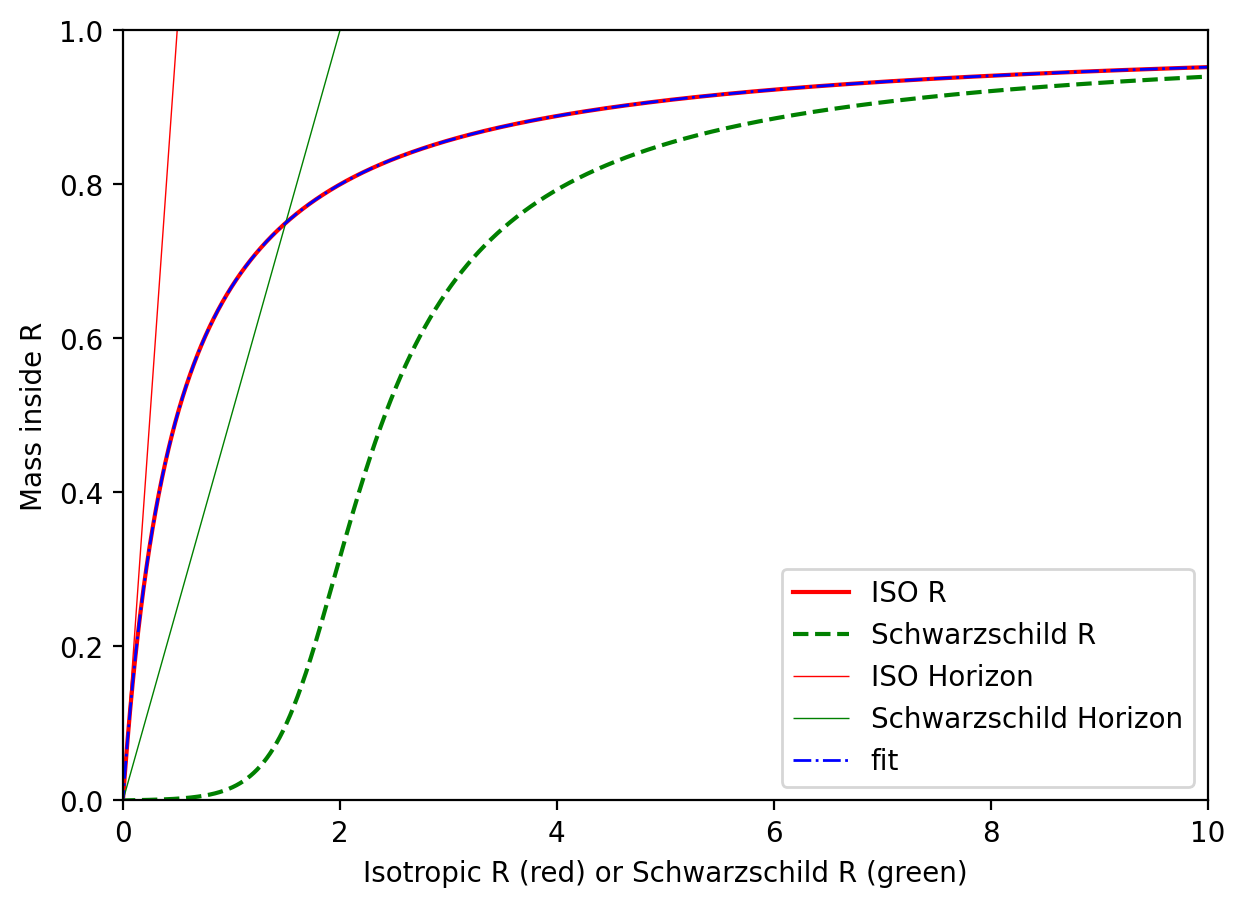
\includegraphics[width=0.70\textwidth]{chapters/images/no-horizons.png}
\caption{Assuming that building the gravitational energy around a 'black hole' requires energy, I find that there is no horizon. In addition, an exact analytical function describing the mass function was found. }
\label{isotropic-energy-hole}
\end{figure}

\begin{figure}
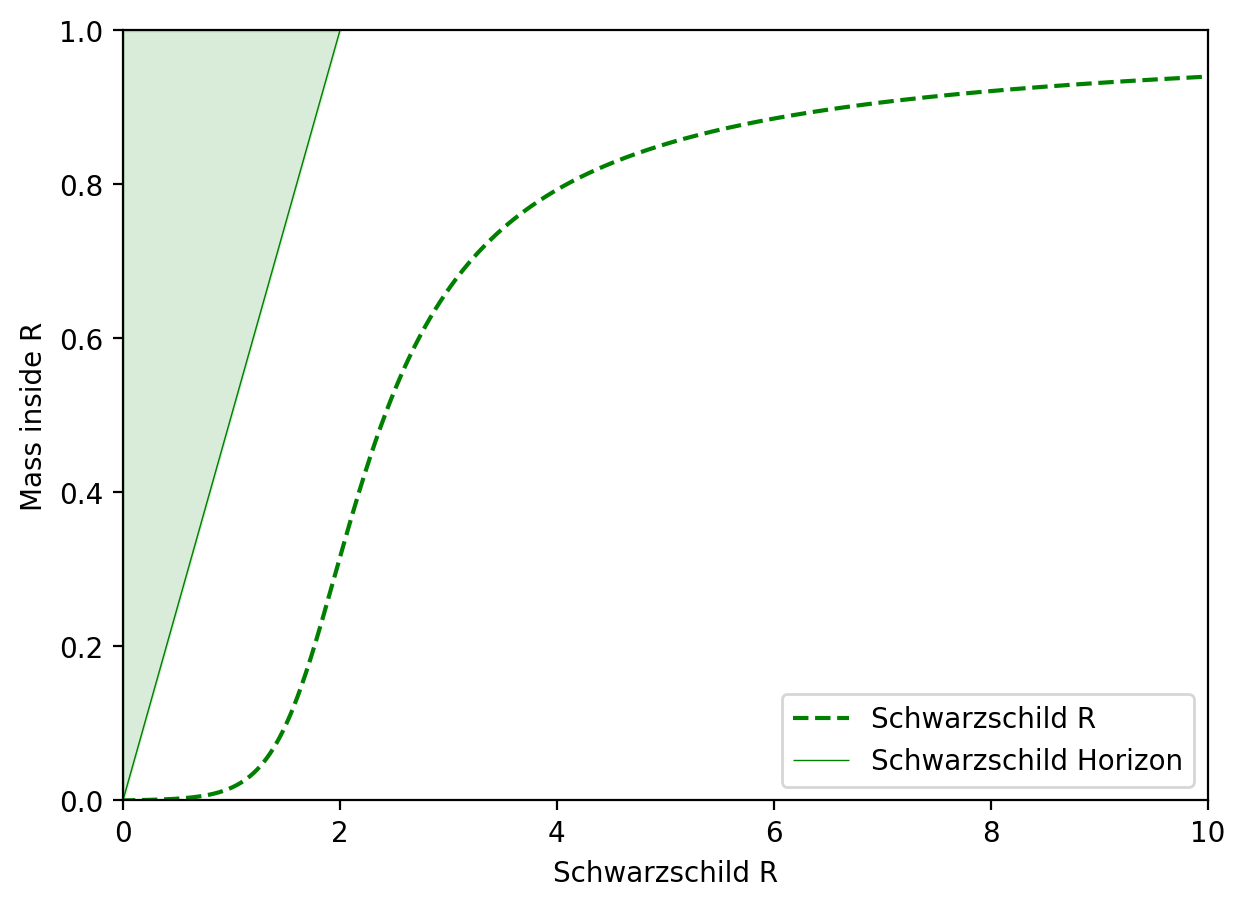
\includegraphics[width=0.70\textwidth]{chapters/images/no-horizons-s.png}
\caption{The same data as in figure \ref{isotropic-energy-hole}, but with Schwarzschild coordinates. The mass at every radius is below the horizon radius for that mass, so there is no event horixon.}
\label{isotropic-energy-hole-s}
\end{figure}



\end{document}
